\title{\vspace{-2.0cm} 60006 - Tutorial 2

Edge Detection, Hough Transform}
\author{
        Xin Wang
}
\date{\today}

\documentclass[12pt]{article}
\usepackage[margin=0.5in]{geometry} 
\usepackage{amsmath} 
\usepackage{graphicx}  
\usepackage[parfill]{parskip}

\graphicspath{{Images/}}

\setlength{\parindent}{0em}

\begin{document}
\maketitle

\section*{Question 1}

The horizontally and vertically flipped kernels are defined as:
$$
 h_{x_{flipped}} = \begin{bmatrix}
     -1 & 0 & 1 \\
     -1 & 0 & 1 \\
     -1 & 0 & 1
 \end{bmatrix} \quad \text{ and } \quad h_{y_{flipped}} = \begin{bmatrix}
    -1 & -1 & -1 \\
    0 & 0 & 0 \\
    1 & 1 & 1
\end{bmatrix} 
$$

\textbf{Question 1.1:} If we use zero padding at the boundary pixels, what is gradient magnitude of the second row
after being convolved by 3x3 Prewitt filter kernels?

Convolution on the second row:
$$
    g_x = f * h_{x_{flipped}} 
$$
$$
\begin{bmatrix}
    12 & 15 & 33 & 51 & 90 & 75 & 21 & -150
\end{bmatrix}
$$
$$
    g_y = f * h_{y_{flipped}} 
$$
$$
\begin{bmatrix}
    0 & 0 & 0 & 0 & 0 & 0 & 0 & 0
\end{bmatrix}
$$

Gradient magnitude:
$$
    g = \sqrt{g_x^2 + g_y^2}
$$
$$
\begin{bmatrix}
    12 & 15 & 33 & 51 & 90 & 75 & 21 & 150
\end{bmatrix}
$$

\textbf{Question 1.2:} If we use replicate padding (padding using the same value as the boundary pixel), what is the
gradient magnitude of the second row?

Convolution on the second row:
$$
    g_x = f * h_{x_{flipped}} 
$$
$$
\begin{bmatrix}
    3 & 15 & 33 & 51 & 90 & 75 & 21 & 6
\end{bmatrix}
$$
$$
    g_y = f * h_{y_{flipped}} 
$$
$$
\begin{bmatrix}
    0 & 0 & 0 & 0 & 0 & 0 & 0 & 0
\end{bmatrix}
$$

Gradient magnitude:
$$
    g = \sqrt{g_x^2 + g_y^2}
$$
$$
\begin{bmatrix}
    3 & 15 & 33 & 51 & 90 & 75 & 21 & 6
\end{bmatrix}
$$

\textbf{Question 1.2:} If we use replicate padding and the 3x3 Sobel filter, what is the result? 

The Sobel filters kernels are defined as:
$$
 h_{x} = \begin{bmatrix}
     1 & 0 & -1 \\
     2 & 0 & -2 \\
     1 & 0 & -1
 \end{bmatrix} \quad \text{ and } \quad h_{y} = \begin{bmatrix}
    1 & 2 & 1 \\
    0 & 0 & 0 \\
    -1 & -2 & -1
\end{bmatrix} 
$$

The horizontally and vertically flipped kernels are defined as:
$$
 h_{x_{flipped}} = \begin{bmatrix}
     -1 & 0 & 1 \\
     -2 & 0 & 2 \\
     -1 & 0 & 1
 \end{bmatrix} \quad \text{ and } \quad h_{y_{flipped}} = \begin{bmatrix}
    -1 & -2 & -1 \\
    0 & 0 & 0 \\
    1 & 2 & 1
\end{bmatrix} 
$$

Convolution on the second row:
$$
    g_x = f * h_{x_{flipped}} 
$$
$$
\begin{bmatrix}
    4 & 20 & 44 & 68 & 120 & 100 & 28 & 8
\end{bmatrix}
$$
$$
    g_y = f * h_{y_{flipped}}
$$
$$
\begin{bmatrix}
    0 & 0 & 0 & 0 & 0 & 0 & 0 & 0
\end{bmatrix}
$$

Gradient magnitude:
$$
    g = \sqrt{g_x^2 + g_y^2}
$$
$$
\begin{bmatrix}
    4 & 20 & 44 & 68 & 120 & 100 & 28 & 8
\end{bmatrix}
$$

\section*{Question 2}

Calculate the gradient direction for the pixel in the centre using the Prewitt filters.
\begin{gather*}
    g_x = f * h_x = 10 \\ 
    g_y = f * h_y = -10
\end{gather*}

Gradient direction:
$$
    \arctan(\frac{g_y}{g_x}) = -45\deg
$$

\section*{Question 3}

The following points appear in an edge map: $(-2, -3), (-1, -1), (0, 1), (1, 3), (4, 9)$.
We would like to use the Hough transform to estimate a line model from the points. 
\begin{itemize}
    \item Find the line model parameters for these points. You can use the
    figure below (abscissa: $m$, ordinate: $b$) to do this.

    \begin{align*}
        (-2,-3) &\rightarrow b = -3 + 2x \\
        (-1,-1) &\rightarrow b = -1 + 1x \\
        (0,1) &\rightarrow b = 1 \\
        (1,3) &\rightarrow b = 3 - x \\
        (4,9) &\rightarrow b = 9 - 4x    
    \end{align*}

    \pagebreak

    \item Please sketch the corresponding lines in the parameter space using the slope intercept form for the line model
    $y = mx + b$, i.e. $b = y - mx$.
    \begin{figure}[h]
        \centering
        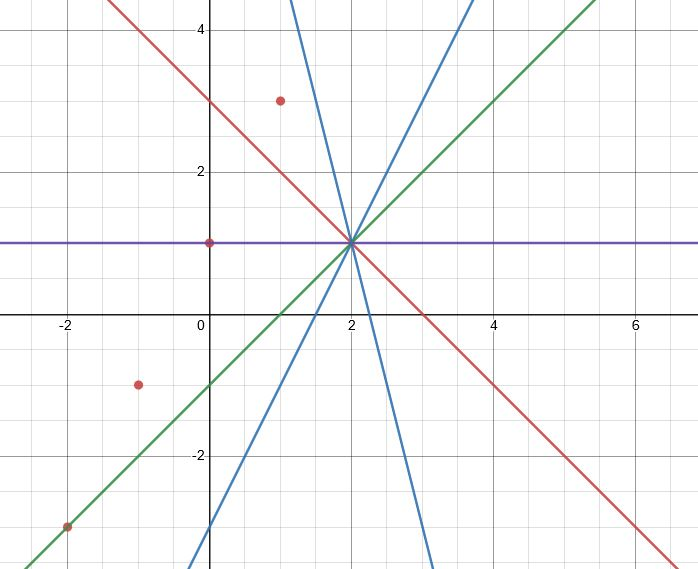
\includegraphics[width=8cm]{Q3.JPG}
    \end{figure}

    The lines sintersect at $(2, 1)$. So the fitted line model is $y = 2x + 1$.
\end{itemize}
 
\section*{Question 4}

Expand the loss function:
$$
    E(\beta) = Y^T - 2X^T \beta^T Y + X^T \beta^T X \beta 
$$

Differentiating:
$$
    \frac{\partial E}{\partial \beta} = -2X^T Y + 2X^T X \beta
$$

To get the optimum, let $\frac{\partial E}{\partial \beta} = 0$:
\begin{align*}
    -2X^T Y + 2X^T X \beta = 0 \\ 
    \beta = \frac{X^T Y}{X^T X}
\end{align*}



\end{document}

  